\section{Experiments}\label{sec:Experiments}
In this section, we validate our system by answering the following questions:

\begin{itemize}
    \item Why use our learning-based line detector instead of classical methods?
    \item The initial reference trajectory can be in collision with the power masts. In this case, can our system safely avoid the power masts?
    \item Does tightly-coupled perception \iros{and action} improve data quality for visual inspection?
\end{itemize}
In addition, we demonstrate our system in the real world on a mock-up power line infrastructure.
The proposed perception-aware MPC runs inside the quadrotor control stack~\cite{foehn2022agilicious}.
\medskip

\textbf{Benefits of our learning-based line detector:}
\begin{figure}[t!]
    \centering
    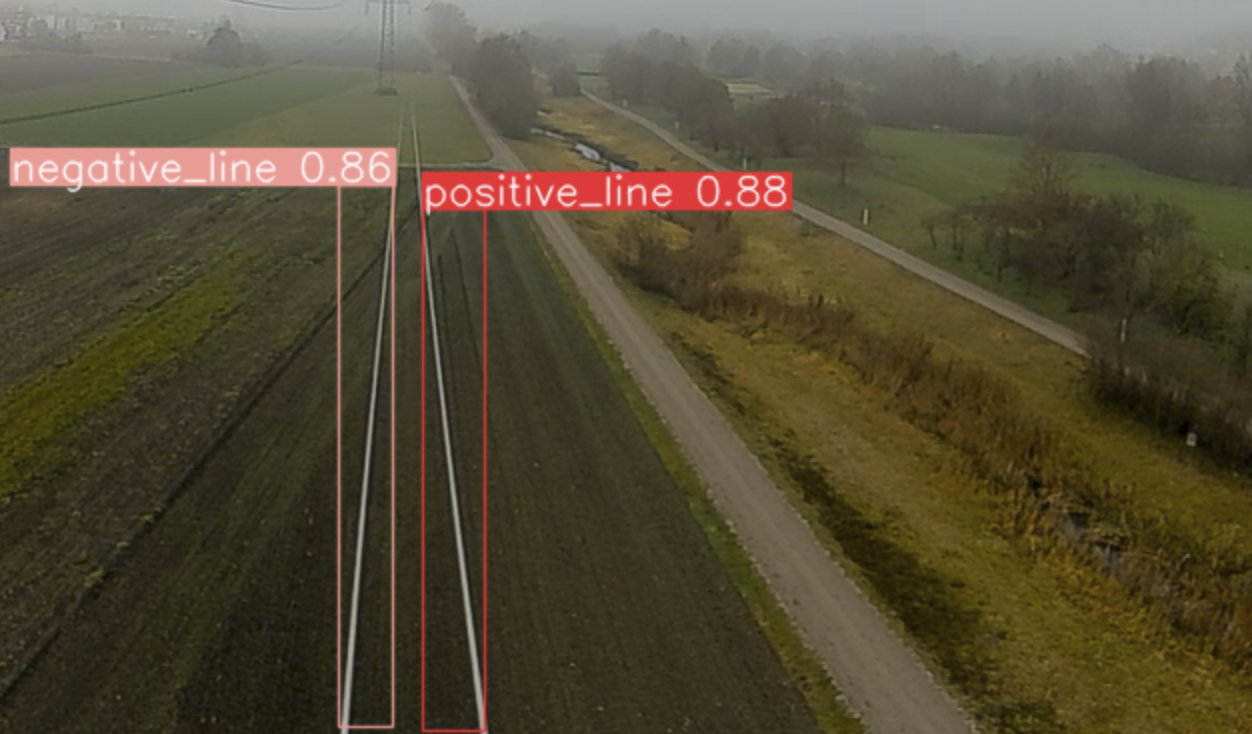
\includegraphics[width=0.98\columnwidth]{figures/real-yolo.png}
    \vspace{0.5ex}
    \caption{A sample result of our line detector validated using a real-world image. Our detector shows correct prediction with high confidence in a challenging real-world scene, despite only being trained with synthesized images.}
    \label{fig:yolo}
    \vspace{-2.5ex}
\end{figure}
In these experiments, we compare the proposed learning-based line detector against a traditional line detector approach based on the Hough transform algorithm~\cite{illingworth1988survey}.
We design a traditional line detection baseline that uses the Canny edge detector algorithm~\cite{bao2005canny} to detect edge features in the image and the Hough transform algorithm to estimate the line parameters.
We also design a probabilistic version of this algorithm, Probabilistic Hough Transform (P-Hough), that runs on a sampled subset of the detected edges.
The dimension of this subset depends on predefined thresholds that vary according to the number of detected edges.
The parameters of the traditional approach were tuned on the training sequences of our simulated power line dataset.
The results on the test sequences are listed in Table~\ref{tab:quant_eval_in}.
We use the metrics proposed in~\cite{zhao2021deep}, which are the Precision, Recall, and the F1 score of the line matching results based on Chamfer distance and EA score~\cite{zhao2021deep}.
Our line detector greatly outperforms the traditional approach.
Generally, it is difficult to find a set of parameters for the traditional approach that generalizes to the different environments of our dataset.
On the contrary, our learning-based detector is able to generalize to all the environments in the dataset.
Furthermore, we demonstrate that our proposed line detector is able to generalize to real-world data without fine-tuning.
Fig.~\ref{fig:yolo} shows the output of the line detector on a real-world power line image recorded onboard a quadrotor. 
We refer the reader to the accompanying video where we include the results of our line detector on the full sequence of images recorded onboard a quadrotor flying above the real-world power lines.
%
\begin{table}[t!]
	\centering
	\begin{tabular}{lcccccccl}
		\toprule
		\textbf{Method}&\multicolumn{3}{c}{\textbf{Chamfer Distance}} & \multicolumn{3}{c}{\textbf{EA Score}}\\
		\midrule
		&P&R&F&P&R&F\\
		Hough&0.70&0.32&0.44&0.46&0.19&0.28\\
		P-Hough&0.26&0.31&0.28&0.10&0.16&0.10\\
		\midrule
		\textbf{Ours}&\textbf{0.92}&\textbf{0.77}&\textbf{0.84}&\textbf{0.93}&\textbf{0.78}&\textbf{0.85}\\
        \midrule
		Improvement (\%)&31&141&91&102&311&204\\
		\bottomrule
	\end{tabular}
    \vspace{1ex}
	\caption{Quantitative evaluation of the performance of the proposed learning-based line detector and of the classical approaches.}

	\label{tab:quant_eval_in}
      \vspace{-2.5ex}

\end{table}
%
We also evaluate the line detection algorithms in terms of the time they need to process a single frame, which we name running time.
Such a running time was computed on a laptop equipped with an Intel Xeon E3-1505M v5 (2.80GHz) CPU and Nvidia Quadro M2000M GPU, and on Nvidia Jetson TX2, which is the computer available onboard our quadrotor platform.
The results are shown in Table~\ref{tab:trad_methods}. 
\iros{
Furthermore, to justify the need for the proposed line detector, we compare our approach against the state-of-the-art models~\cite{pan2018spatial, tabelini2021keep, liu2021condlanenet, li2019line, chen2019pointlanenet} for pixel-wise line detection regarding the computation time.
\begin{table}[b]
	\centering
	\begin{tabular}{lcccl}
		\toprule
		\textbf{Method}  & \textbf{Run Time [ms]} & \textbf{GFlops}  \\
		\midrule
		SCNN~\cite{pan2018spatial} & 133.33 & 328.4 \\
		LaneATT~\cite{tabelini2021keep} & 38.46 & 70.5\\
		CondLaneNet~\cite{liu2021condlanenet} & 17.18 & 44.8\\
		Line-CNN~\cite{li2019line} & 27.93 & - \\
		PointLaneNet~\cite{chen2019pointlanenet} & 14.08&-\\
		\midrule
		\textbf{Ours} & \textbf{1.80} & \textbf{0.0042}\\ 
		\bottomrule
	\end{tabular}
 \vspace{1ex}
	\caption{\iros{Comparison of the state-of-the-art line detection methods with respect to their inference speeds and operation numbers. Our approach outperforms the state-of-the-art methods in terms of computational efficiency, All experiments use the same input image size of $512\times512$ on Nvidia GeForce RTX 2080Ti GPU.}}
	\label{tab:learn_methods}
  \vspace{-3.5ex}

\end{table}
As shown in Table \ref{tab:learn_methods},
the high latency of these models makes them unsuitable for real-time deployment onboard resource-constrained platforms such as quadrotors. 
The high latency is mainly because these methods predict pixel-wise segmentation, which is not needed in our use case.}\\


\begin{figure}[t!]
    \centering
    \vspace{-1ex}
    \begin{tikzpicture}
            \node[inner sep=0pt] (pic) at (0,0){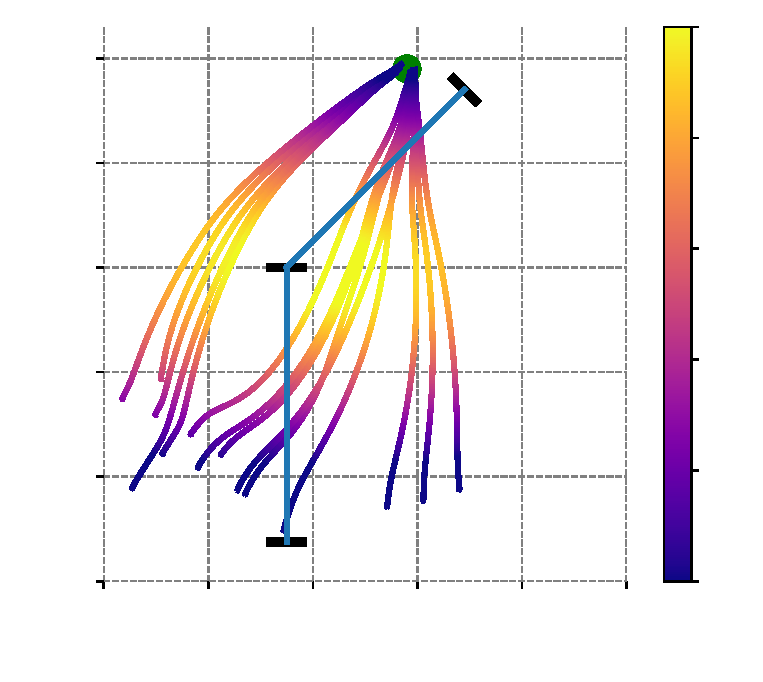
\includegraphics[width=1.0\columnwidth]{figures/fig_clean.pdf}};
            % x coodinate
            \node[inner sep=0pt] at (-3.15, -3.1){0};
            \node[inner sep=0pt] at (-1.96, -3.1){2};
            \node[inner sep=0pt] at (-1.96+1.19, -3.1){4};
            \node[inner sep=0pt] at (-1.96+1.19*2, -3.1){6};
            \node[inner sep=0pt] at (-1.96+1.19*3, -3.1){8};
            \node[inner sep=0pt] at (-1.96+1.19*4, -3.1){10};

            \node[inner sep=0pt] at (-1.96+1.19*1.5, -3.5){$x$ [m]};


            % y coordinate
            \node[inner sep=0pt] at (-3.5, -2.75){0};
            \node[inner sep=0pt] at (-3.5, -2.75 + 1.19){2};
            \node[inner sep=0pt] at (-3.5, -2.75 + 1.19*2){4};
            \node[inner sep=0pt] at (-3.5, -2.75 + 1.19*3){6};
            \node[inner sep=0pt] at (-3.5, -2.75 + 1.19*4){8};
            \node[inner sep=0pt] at (-3.5, -2.75 + 1.19*5){10};
            \node[inner sep=0pt, rotate=90] at (-3.9, -2.75 + 1.19*2.5){$y$ [m]};

            % colorbar
            \node[inner sep=0pt] at (4, -2.7) {0.0};
            \node[inner sep=0pt] at (4, -2.7+1.25) {0.2};
            \node[inner sep=0pt] at (4, -2.7+1.25*2) {0.4};
            \node[inner sep=0pt] at (4, -2.7+1.25*3) {0.6};
            \node[inner sep=0pt] at (4, -2.7+1.25*4) {0.8};
            \node[inner sep=0pt] at (4, -2.7+1.25*5) {1.0};

            %ABC
            \node[inner sep=0pt] at (-0.5, -2.3) {\large A};
            \node[inner sep=0pt] at (-1.45, 0.85) {\large B};
            \node[inner sep=0pt] at (1.4, 2.9) {\large C};

            %Goal
            \node[inner sep=0pt] at (-0.2, 3.5) {Goal};


    \end{tikzpicture}
    \caption{Visualization of the flown trajectories color-coded according to the values of $\alpha$, c.f. Sec.~\ref{sec:perception_aware_mpc}.
    Our MPC is able to find collision-free trajectories starting from non-collision-free reference trajectories.}
    \label{fig:sim}
\end{figure}
\noindent
\textbf{Robustness to unknown location of the power masts: }
\begin{table}[t!]
	\centering
	\begin{tabular}{lcccl}
		\toprule
		\textbf{Method}  & \textbf{Run Time Laptop [ms]} & \textbf{Run Time TX2 [ms]} \\
		\midrule
		Hough &7.19&18.52\\
        \textbf{P-Hough}  &\textbf{4.61}&\textbf{16.13}  \\
		\midrule
		Ours& 4.69& 20.83\\ 
		\bottomrule
	\end{tabular}
    \vspace{1ex}
	\caption{Running time, i.e. time required to process a single image, of the proposed learning-based line detection algorithm and of the classical approaches.}
    \vspace{-3.5ex}
	\label{tab:trad_methods}
\end{table}
Generally, the location of the power masts is either unavailable or GPS coordinates with errors up to several meters ($>$ 10) are available.
For this reason, it is not possible to plan a collision-free reference trajectory.

In this experimental setting, we evaluate the performance of our system in the case where the initial reference trajectory is in collision with the power masts.
We run our tests within the Flightmare simulation environment and assume that the MPC has access to the ground truth obstacle position and only vary the reference trajectory.
We designed an environment with 3 power masts (labelled A, B, C) as shown in Fig.~\ref{fig:sim}.
We randomly sampled 100 starting points in a rectangular region of size 8$\times$3 m in the vicinity of the power mast A (the center of A is located in the middle of the bottom edge of this rectangular region).
The endpoint is fixed 1 m away from the left side of the power mast C.
The reference trajectory given to the MPC is a straight line connecting the starting and end points with no yaw change.
Some of these reference trajectories are in collision with the power mast B.
Our system achieves a 100\% success rate, i.e. no collision with the power masts.
We show in Fig.~\ref{fig:sim}, 13 flown trajectories.\\

\noindent
\textbf{Benefits of tightly-coupling perception and action:}
In this experiment, we evaluate the benefits of tightly-coupling perception, planning, and control in terms of visibility of the power lines compared to the classical MPC formulation (c.f. Eq.~\ref{eq:classical_mpc}).
We use the proposed learning-based line detector and assume that the MPC has access to the ground-truth position of the power masts.
We use the similarity score $\mathcal{S}$ as the evaluation metric, which is defined as:
\begin{equation}
	\mathcal{S}_\theta = 1- \frac{2\theta}{\pi},\;
	\mathcal{S}_d = 1 - \frac{h}{\sqrt{w^2 + l^2}},\;
	\mathcal{S} = (\mathcal{S}_\theta \cdot \mathcal{S}_d)^2
 \label{eq:sim_score}
\end{equation}
%
%
%

%
\noindent
where $\theta$ is the normalized angular distance between the detected and the reference line, and $h$ is the normalized distance between the center points of the lines (c.f. Fig.~\ref{fig:lineeval}).
The quantity $h$ is normalized by the length of the image diagonal, where $w$ and $l$ are the image width and height, respectively.
We run the experiments on the testing sequences of our dataset which are from 4 different environments: Simple, Warehouse, Forest, and Village.
The results are in Table~\ref{tab:eval}. 
Our perception-aware MPC improves the line visibility on average by 40\%.

In addition, we evaluated the run time of our perception-aware MPC formulation (c.f. Eq.~\ref{eq:perception_aware_mpc}), the classical MPC formulation, an MPC including the only line tracking objective (Tracking MPC), and, an MPC including the only collision avoidance objective (Avoidance MPC).
We report the update and solver time when running the algorithms on an Nvidia Jetson TX2 platform, which is the computer onboard our quadrotor.
The update time is the period of time between two consecutive control commands.
The solver time is the period of time taken by the solver to optimize the MPC objective.
The results are shown in Table~\ref{tab:mpc_run_time}.
Our proposed MPC requires more computational time than the classical formulation mainly due to the collision objective.
However, the update is fast enough to deploy the proposed MPC on a real quadrotor.
\begin{figure}[t!]
    \centering
    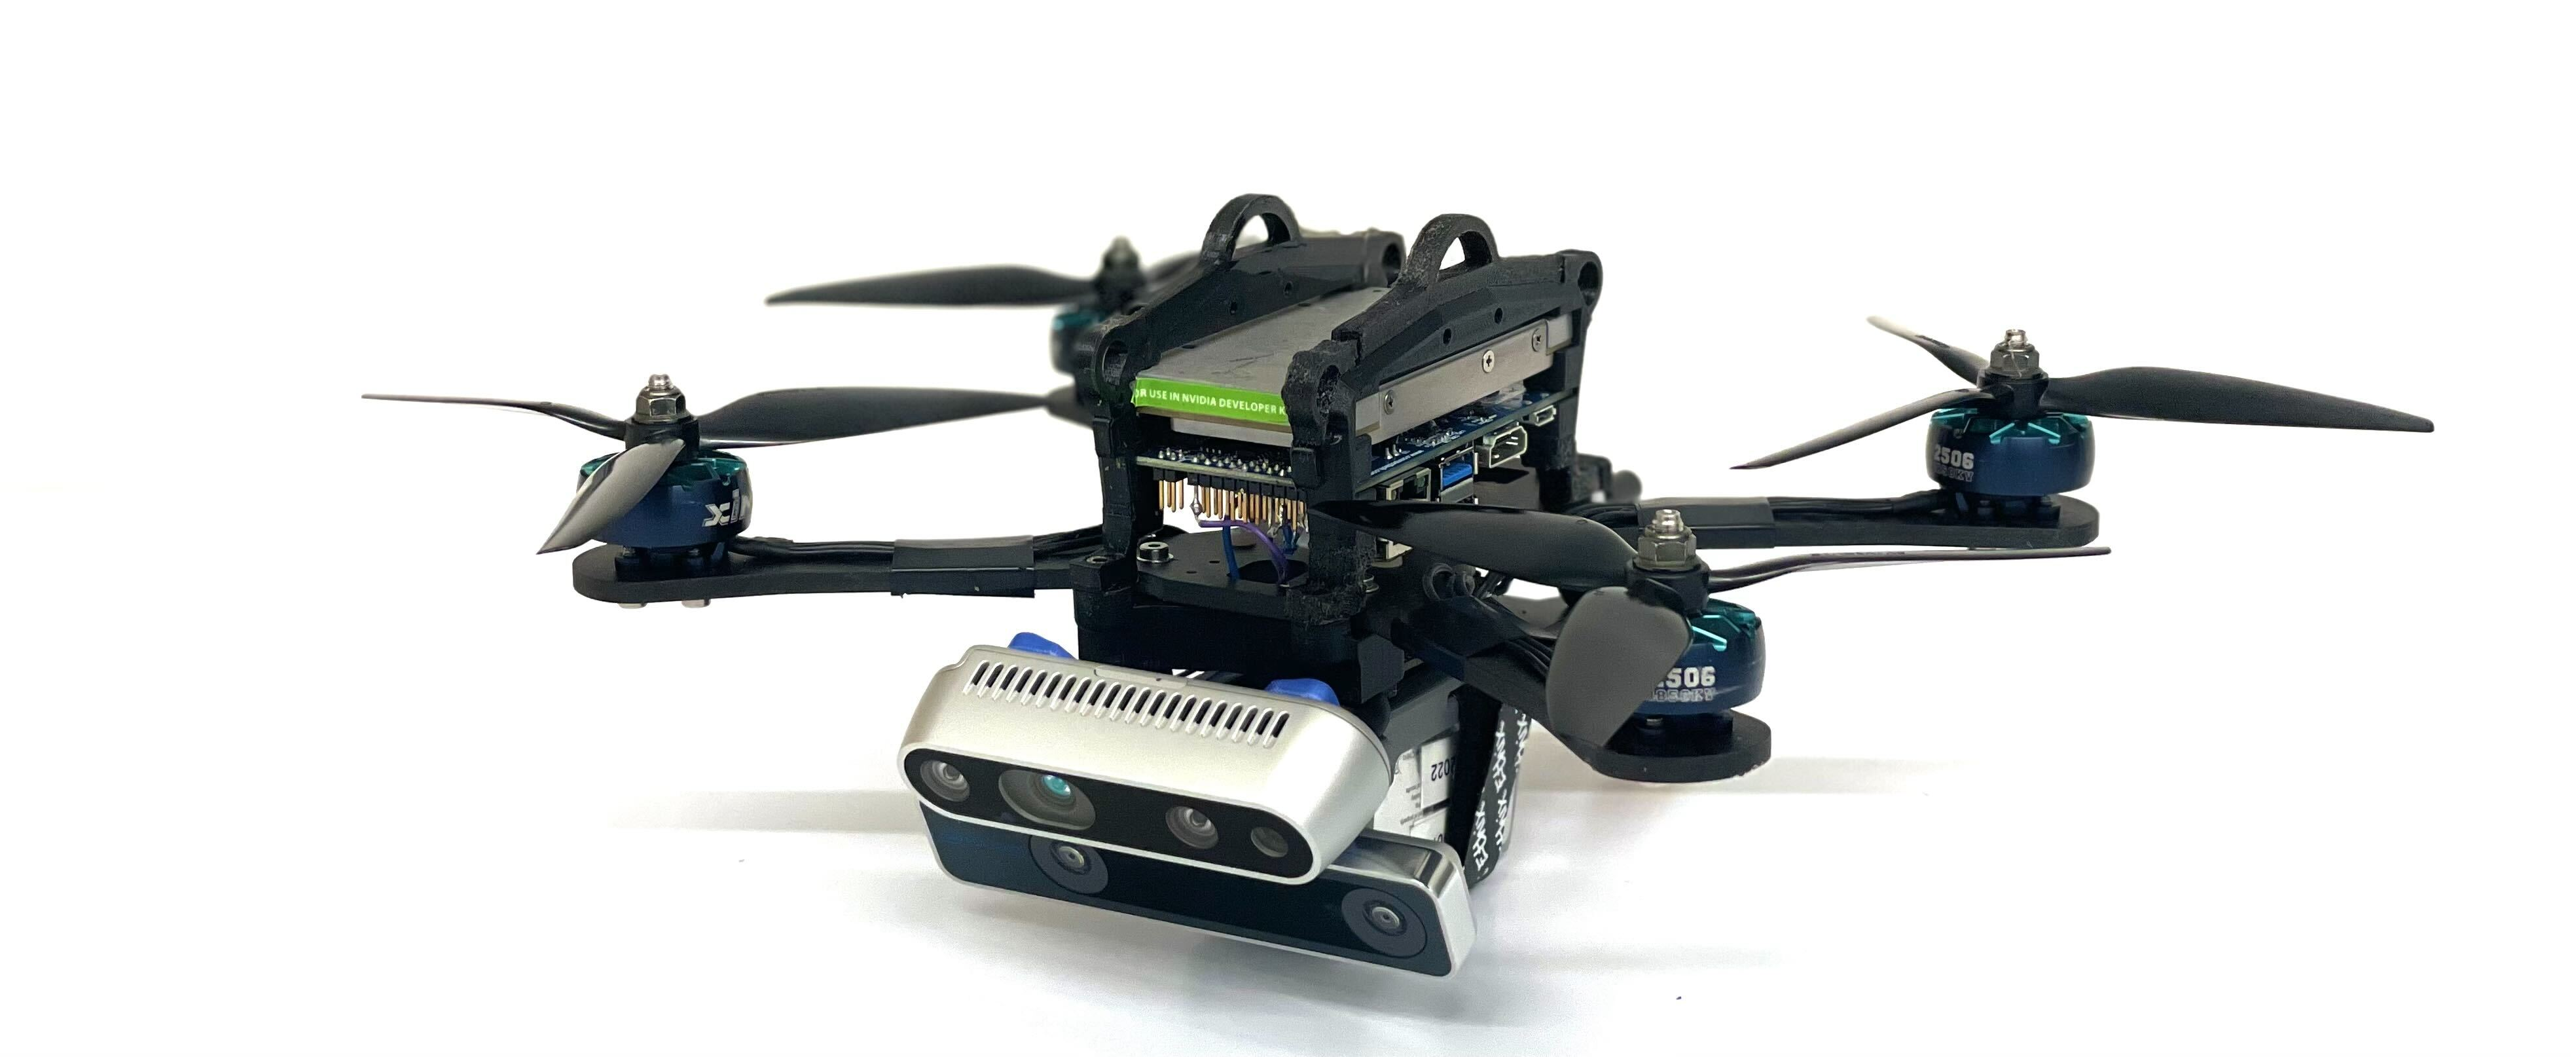
\includegraphics[width=0.95\columnwidth]{figures/hardware.jpg}
    \caption{Quadrotor used in real-world experiments.}
    \label{fig:frame}
    \vspace{-2ex}
\end{figure}


\begin{table}[t!]
	\centering
	\begin{tabular}{lccccccl}
		\toprule
		&\textbf{Simple}  & \textbf{Warehouse} & \textbf{Forest} & \textbf{Village}& \textbf{Mean}      
  \\
  \midrule
		\textbf{Our MPC}  & \textbf{0.74} & \textbf{0.63} & \textbf{0.61} & \textbf{0.67} & \textbf{0.67}\\
		Classical MPC  & 0.53 & 0.49 & 0.44 & 0.45 & 0.48\\
		\bottomrule
	\end{tabular}
	\vspace{1ex}
	\caption{Quantitative comparison of the proposed perception-aware MPC (Eq.~\ref{eq:perception_aware_mpc}) against the classical MPC formulation (Eq.~\ref{eq:classical_mpc}). The evaluation metric refers to the visibility of the line (Eq.~\ref{eq:sim_score}).}
	\vspace{-2.5ex}
	\label{tab:eval}
\end{table}

%
\begin{table}[b!]
	\centering
	\begin{tabular}{lcccl}
	\toprule
	&\textbf{Update Time [ms]}&\textbf{Solver Time [ms]}\\
	\midrule
	Classical MPC&0.88$\pm$0.27 & 0.65 $\pm$0.01\\
	Tracking MPC & 0.99$\pm$0.03 & 0.75 $\pm$ 0.02\\
	Avoidance MPC &7.31$\pm$3.15&7.14 $\pm$3.01\\
	Our MPC&7.90$\pm$3.63&7.67$\pm$3.62\\
	\bottomrule
\end{tabular}
\vspace{1ex}
\caption{Comparison of multiple MPC formulations with respect to their update time and solver time.}
\vspace{-2.5ex}

\label{tab:mpc_run_time}
\end{table}
\textbf{Real-world deployment:}
We deploy our system on a quadrotor equipped with an Intel Realsense T265 tracking camera and an Intel Realsense D435i depth camera.
The onboard computer is an Nvidia Jetson TX2.
Detailed information about our quadrotor platform is in~\cite{foehn2022agilicious}.
We use the VIO algorithm from the tracking camera to obtain an estimate of the 6-DoF pose of the quadrotor and the depth camera to obtain RGB images for the line detection algorithm and depth measurements for the collision avoidance algorithm.
All the components of our system run on the onboard computer in real-time.
We set up a mock-up power line environment featuring 3 power masts.
The distance between each pair of power masts is 7.5 m.
A top view of the power environment including a trajectory flown by our quadrotor is in Fig~\ref{fig:catcheye}.
We run several experiments with different starting positions sampled in the vicinity of mast A.
\iros{In all the experiments, the proposed MPC does not have access to the ground-truth location of the power lines and power masts.
For this reason, a classical MPC approach without perception awareness is not a suitable solution.}
We demonstrate that our quadrotor is able to track the power line by adapting its heading (c.f., Fig~\ref{fig:catcheye}) and to avoid the power masts.
We refer the reader to the accompanying video for the visualization of these experiments.
